\documentclass[12pt]{../manual}
%____________________________________________________________________________
%
%	TITLE AND TABLE OF CONTENTS
%____________________________________________________________________________
\begin{document}
\makeheader{Lab 6}{Fall 2019} % Change Semester and Year as needed
\begin{center}
\textbf{\huge ECE 230L - LAB 6}\\~\\
\textbf{\large BASIC DIGITAL CIRCUITS}\\~\\
\rule{6.5in}{0.5mm}\\
\end{center}

\tableofcontents

\listoffigures

\newpage
%____________________________________________________________________________
%
%	BODY
%____________________________________________________________________________
\section{Objectives of this Laboratory}
The objectives of this laboratory session are as follows:
\begin{itemize}
\item Measure the static and switching characteristics of discrete (transistors, resistors, and capacitors) MOS inverter circuits,
\item Measure the static voltage-transfer characteristics of CMOS NOR and NAND gates,
\item Determine experimentally the truth tables of CMOS integrated-circuit gates, and
\item Measure the switching characteristics of CMOS NOR and NAND gates
\end{itemize}

\section{Discrete Diode Logic OR and AND Gates}
Diodes can be used to significantly reduce circuit cost, complexity, and save precious board space. By implementing discrete-device logic instead of using OR and AND gates, whole integrated circuits (ICs) can be replaced in a circuit. In general, ICs with 50\% or fewer gates being used stand to gain by being replaced by discrete components. Diode logic takes advantage of the diode properties to build useful circuits that can reduce component count and simplify circuits. A few simpler components can be inserted to perform the same function of large integrated circuits more cheaply and more directly. Often, it is more convenient to build a logic gate then use a pre-manufactured chip. When more than a few inputs are desired, building your own logic gates can be the only way to get the desired number. For instance, a 7-input OR gate is easily implemented just by adding more diodes to a basic 2-input gate. You may not always have the ICs that you need available, and ordering them and then waiting for the delivery takes time. You will always have resistors and diodes, and this is another reason for using logic gates made from discrete components.

\newpage
\subsection{Diode OR Gate}
Consider the diode as a simple switch. It is closed (ON) when the voltage on the anode or p-side is higher than that on the cathode or n-side. Current flows in the direction of the arrow in the diode's schematic symbol. The logic symbol of an OR gate and its discrete diode implementation are shown in Figure \ref{fig:OR}. In an OR gate, the output is `1' if either of the inputs are `1'. In other words, if either of the inputs has a high voltage, its diode will conduct and current will flow to the output. A high voltage will appear across the resistor, equal to the input voltage minus a voltage drop across the silicon diode. If both of the inputs are `0', then neither of the diodes will conduct and the gate?s output voltage will be zero. 

\begin{itemize}
\item[$\square$] Wire the diode OR gate using 1N4148 Si diodes on a breadboard and verify its truth table by applying 0 and \SI{5}{\volt} (4 combinations) to the inputs A and B. Measure the value of the output voltage. Note the diode voltage drop and its effect on the output voltage.
\end{itemize}

\begin{figure}[ht!]
\centering
\begin{tabular}{m{5cm} m{5cm}}
\begin{circuitikz}[american]
\draw (0,0) 	node[american or port, name=A] {};
\draw (A.in 1) 	to[short, -o] ++(-0.5,0) node[left] {A};
\draw (A.in 2) 	to[short, -o] ++(-0.5,0) node[left] {B};
\draw (A.out) 	to[short, -o] ++(0.5,0) node[right] {C};
\end{circuitikz} &
\begin{circuitikz}[american]
\draw (0,0) 	node[left] {A}
				to[D*, o-*] ++(3,0) 
				to[short, -o] ++(2,0) node[right] {C};
\draw (3,0) 	to[short] ++(0,-1)
				to[R, l=$R$, a=\SI{10}{\kilo\ohm}] ++(0,-2) node[ground, below] {};
\draw (0,-1)	node[left] {B}
				to[D*, o-*] ++(3,0);
\end{circuitikz}
\end{tabular}
\caption{OR Gate Symbol and Discrete Diode Implementation}
\label{fig:OR}
\end{figure}

Note that `$+$' is used to represent the OR operation. Hence, in Figure \ref{fig:OR} we have 
\begin{align}
C = A + B.
\end{align}

\newpage
\subsection{Diode AND Gate}
Consider the diode AND gate shown in Figure \ref{fig:AND}. Its circuit is similar to the OR-gate circuit except that the diode connections (anodes and cathodes) are switched, and the resistor is connected to a power supply of \SI{5.0}{\volt}, instead of ground. The output of an AND gate is `1' only if both inputs are `1'. In the diode implementation, if either input is `0', then the diode will conduct and the output voltage will be effectively shorted (through the diode) to ground. If both inputs are `1' , then neither of the diodes will be conducting and the output voltage will be \SI{5.0}{\volt} (logical `1') because nearly all the voltage drops across the \SI{10}{\mega\ohm} resistor. This operation yields the desired result. Note that again, due to the voltage drop across a conducting silicon PN-junction diode, the actual `low' output voltage is higher than the `low' voltage of \SI{0}{\volt} applied at the input of the gate.

\begin{itemize}
\item[$\square$] Wire the diode AND gate using 1N4148 Si diodes on a breadboard and verify its truth table by applying 0 and \SI{5}{\volt} (4 combinations) to the inputs A and B. Measure the output voltage. Note the diode voltage drop and its effect on the output voltage.
\end{itemize}

\begin{figure}[ht!]
\centering
\begin{tabular}{m{5cm} m{5cm}}
\begin{circuitikz}[american]
\draw (0,0) 	node[american and port, name=A] {};
\draw (A.in 1) 	to[short, -o] ++(-0.5,0) node[left] {A};
\draw (A.in 2) 	to[short, -o] ++(-0.5,0) node[left] {B};
\draw (A.out) 	to[short, -o] ++(0.5,0) node[right] {C};
\end{circuitikz} &
\begin{circuitikz}[american]
\draw (0,0) 	node[left] {A}
				to[D*, invert, o-*] ++(3,0) 
				to[short, -o] ++(2,0) node[right] {C};
\draw (3,0) 	to[R, a=$R_1$, l=\SI{10}{\kilo\ohm}] ++(0,2) node[vdd, above] {$V_{\mathrm{DD}}$};
\draw (3,0) 	to[short] ++(0,-1)
				to[R, l=$R_2$, a=\SI{10}{\mega\ohm}] ++(0,-2) node[ground, below] {};
\draw (0,-1)	node[left] {B}
				to[D*, invert, o-*] ++(3,0);
\end{circuitikz}
\end{tabular}
\caption{AND Gate Symbol and Discrete Diode Implementation}
\label{fig:AND}
\end{figure}

Note that `$\cdot$' is used to represent the AND operation. Hence, in Figure \ref{fig:AND} we have 
\begin{align}
C = A \cdot B.
\end{align}

\newpage
\section{Discrete MOS Inverter Circuit}
An inverting function cannot be implemented with diodes and resistors alone. A transistor is needed to provide the inverting action. In this lab, you will use the BS170 N-type Metal Oxide Semiconductor Field Effect Transistor (NMOSFET). If the voltage present at the gate of the transistor is above \SI{0.7}{\volt} (high), the transistor will conduct, reducing the output voltage to logical `0'. If the input voltage is logical `0' (low), then the transistor does not conduct, and zero voltage drops across the load resistor which results in the output voltage being `1'. A current-limiting resistor at the gate is always needed, otherwise excessive gate current might destroy the transistor. The circuit used in the electrical characterization of the MOS inverter with a resistive load is shown in Figure \ref{fig:MOS}. Digital integrated circuits are circuits based on the principles of Boolean algebra. The binary logic variables in this algebra can assume only one of two possible values which are called the logical `0' and `1' levels. In the electronic circuit implementation of Boolean algebra, these variables correspond to the values designated by the voltages $V_\mathrm{OL}$ and $V_\mathrm{OH}$.

\begin{figure}[ht!]
\centering
\begin{tabular}{m{5cm} m{5cm}}
\begin{circuitikz}[american]
\draw (0,0) 	node[american not port, name=A] {};
\draw (A.in 1) 	to[short, -o] ++(-0.5,0) node[left] {A};
\draw (A.out) 	to[short, -o] ++(0.5,0) node[right] {B};
\end{circuitikz} &
\begin{circuitikz}[american]
\draw (0,0)		node[nigfete, solderdot, name=N]{};
\ctikzset{diodes/scale=0.3}
\draw ($(N.S) + (0,0.2)$) to[short,*-] ++(0.5,0)
			to[zzD*] ++(0,1.15)
			to[short, -*] ++(-0.5,0);
\draw (N) circle [radius=25pt];
\draw ($(N) + (0.9,0)$) node[right] {BS170};
\draw (N.S)	to[short] ++(0,-1) node[ground,  below] {};
\draw (N.D) to[short, -*] ++(0,0.5) node[name=A] {}
			to[short, -o] ++(1.5,0) node[right] {B};
\draw (A) 	to[R, l=$R_L$, a=\SI{240}{\kilo\ohm}] ++(0,2) node[vdd] {$V_\mathrm{DD}$};
\draw (N.G) to[short, -o] ++(-1,0) node[left] {A};
\end{circuitikz}
\end{tabular}
\caption{Inverter Gate Symbol and Discrete Diode Implementation}
\label{fig:MOS}
\end{figure}

We usually denote negation with a bar above a character. Hence, in Figure \ref{fig:MOS} we have 
\begin{align}
B = \overline{A}
\end{align}

The static voltage and switching characteristics of an inverter can be characterized and serve as a measure of the inverter's overall performance. The voltages $V_\mathrm{OL}$ and $V_\mathrm{OH}$ are always between 0 and $V_\mathrm{DD}$. The static voltage characteristics of an inverter is shown in Figure \ref{fig:stat}. The switching characteristics of an inverter is shown in Figure \ref{fig:switch}.

\begin{enumerate}
\item Wire the diode Inverter gate using a BS170 MOSFET on a breadboard and verify its
truth table by applying 0 and 5 V (2 combinations) to the input A. Measure the value of
the output voltage. Note the voltage drops across the inverter circuit and their effect on
the output voltage.
\item Using LabVIEW, measure the static voltage-transfer characteristics (SVTC)
VOUT(VIN) for this inverter implemented with the NMOSFET BS170, RL = 240 k?,
and VDD = 5 V. Determine VOL and VOH.
\item Measure the static power-supply-current IDD (VIN ) when VIN = VOL and when VIN
= VOH (both for RL = 240k) (2 cases). Calculate the static power dissipation in this
inverter for VIN = VOL and VIN = VOH. (2 cases) (Hint: P = IV.)
\item Measure the output-voltage waveform vOU T (t) for a square-wave input-voltage
waveform with VPP = 5V and f = 1 kHz obtained from the function generator. Observe
the input and output waveforms on the oscilloscope simultaneously. Determine the
high-to-low transition time (tp.HL) and the low-to-high transition time (tp.LH). Turn up the
input frequency of the square wave keeping the maximum input voltage equal to VPP =
5V. At what frequency does the output waveform begin to degrade? Be as quantitative
as possible.
\end{enumerate}

\begin{figure}[ht!]
\centering
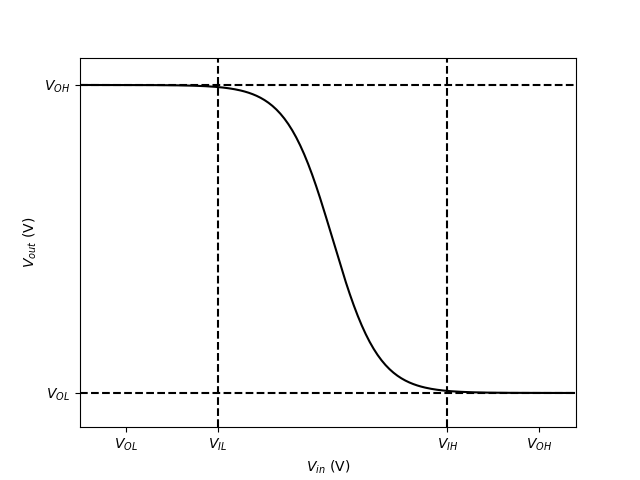
\includegraphics[width=0.7\textwidth]{staticCharInv.png}
\caption{Static Voltage Characteristics of Inverter Circuit}
\end{figure}

\newpage
\section{Exploration}
In this exploration, you will use what you have learned about discrete logic circuits to complete the following:
\begin{enumerate}
\item Build a NAND gate from the combination of discrete AND gates using diodes and Inverter gates using NMOSFET transistors.
\item One very useful application of an Inverter gate is the Inverter Ring Oscillator shown in Figure \ref{fig:ring}. You will build a self-sustaining Ring Oscillator and measure its output square-wave frequency. (A similar circuit can be built using NAND gates chained together. You have all the knowledge you need to build this circuit, too. Hint: to build a Ring Oscillator with NAND gates, one of the two inputs needs be set to Ground. Most designers choose either the A or B input to be grounded for each NAND gate in the chain in this application.)
\item (Optional) Another very useful implementation of NAND gates is the Debounced Switch or SR Latch. A Debounce Switch prevents pushbutton switching events from triggering more than On/Off occurrence in a circuit. Deboucing inputs is critical in many logic circuit applications. A Debounce Swtich or SR Latch can be completely constructed using discrete NAND gate logic when wired as shown in Figure \ref{fig:SR}. This exercise is left as an optional activity.
\end{enumerate}

\subsection{Discrete NAND Gate}
Using a combination of the AND and NOT gates built above, build a discrete NAND gate. Draw a circuit diagram of the circuit you designed and verify the NAND gate truth table. 

\begin{figure}[ht!]
\centering
\begin{circuitikz}[american]
\draw (0,0)		node[american nand port, name=A] {};
\draw (A.in 1) 	to[short, -o] ++(-0.5,0) node[left] {A};
\draw (A.in 2) 	to[short, -o] ++(-0.5,0) node[left] {B};
\draw (A.out) 	to[short, -o] ++(0.5,0) node[right] {C};
\end{circuitikz}
\caption{NAND Gate Symbol}
\label{fig:NAND}
\end{figure}

\newpage
\subsection{Ring Oscillator}
The propagation delay of a switching circuit is a measure of the maximum speed or minimum time
for an input change to pass to the device?s output. Measurements in this mode are made by setting
up an odd number of inverters or inverting gates in a ring, that is, with the output of one inverter
connected to the input of the next inverter. In this mode, a logic steady-state cannot be reached.
The results is a passing along of the logic mismatch?a form of oscillation.
To measure the propagation delay of the discrete inverter built above, arrange an odd number of
inverters (at least 3) in series. No input excitation at the first inverter is needed; the circuit should
oscillate when the inverters are on (i.e. when VDD is applied to each discrete MOSFET inverter).
The output of the Ring Oscillator should be a square wave of amplitude 0 to VDD.

\begin{figure}[ht!]
\centering
\begin{circuitikz}[american]
\draw (0,0) 	node[american not port, name=A] {};
\draw (2,0) 	node[american not port, name=B] {};
\draw (4,0) 	node[american not port, name=C] {};
\draw (A.out)	-- (B.in);
\draw (B.out) 	-- (C.in);
\draw (C.out) 	to[short, -o] ++(2,0);
\draw ($(C.out) + (1,0)$) 	to[short, *-] ++(0,-2) node[name=D] {}
				to[short] ($(D -| A.in) + (-1,0)$)
				to[short] ++(0,2)
				to[short] (A.in);
\end{circuitikz}
\caption{Ring Oscillator Using 3 Inverters}
\label{fig:ring}
\end{figure}

\begin{enumerate}
\item Build the Ring Oscillator in Figure \ref{fig:ring} using an odd number of the discrete NMOSFET BS170 Inverters shown in Figure \ref{fig:MOS}. Observe the output waveform. Notice that no input excitation at the first inverter is needed; the circuit should oscillate at a high frequency when the inverters are on (i.e. when VDD is applied to each discrete MOSFET inverter). Zoom out to view at least 4 periods of the ring oscillator output when determining its period of oscillation.
\item Measure the period of the ring oscillator output square wave. This period is the time required for the logic transition to propagate around all three devices.
\item The transition or propagation time for one gate in this ring oscillator is one-third of the observed period when 3 inverters are used. Determine the transition time of one of the inverters built by dividing the total transition time by 3. (More accurate transition times can be obtained by using additional odd numbers of inverters for this measurement.)
\end{enumerate}

\newpage
\subsection{(Optional) Debounced Switch}
In many applications, especially in digital circuits, you need a manual switch to
set the logic state at some point in the circuit. The issue is that switch can often
``bounce'' upon actuation. A bouncy switch is one that produces multiple
switching operations in a single button press. This leads to a rapid series of
alternating logic states for a few milliseconds while the switch contact is
stabilizing. The bounce is due to inductive ringing rather than mechanical
toggling. We use an SR latch to debounce the switch in hardware by latching
the state of the switch as a digital signal. Once the ringing stops, we can safely
assume that the signal has been latched successfully.

\begin{enumerate}
\item Place a double-pole single-throw switch on a breadboard.
\item Construct the circuit shown in Figure \ref{fig:DPST} and power it with $+\SI{5}{\volt}$.
\item Observe the switch output on an oscilloscope when the input switch is
toggled ``On.'' Capture an occurrence of the switch bouncing phenomenon on the oscilloscope screen and save it.
\end{enumerate}

\begin{figure}[ht!]
\centering
\begin{circuitikz}[american]
\draw (0,0)		node[cute spdt down arrow, rotate=90, name=A] {};
\draw (A.in)	node[ground, below] {};
\draw (A.out 1)	to[short, -*] ++(-1,0) node[name=B] {}
				to[R, l=$R_1$, a=\SI{1}{\kilo\ohm}] ++(0,3) node[vdd] {$V_\mathrm{DD}$};
\draw (B)		to[short] (B |- A.in) node[ground, below] {};
\draw (A.out 2)	to[short, -o] ++(3,0) node[right] {Out};
\draw ($(A.out 2) + (1,0)$) to[R, l=$R_2$, a=\SI{1}{\kilo\ohm}, *-] ++(0,3) node[vdd] {$V_\mathrm{DD}$};
\end{circuitikz}
\caption{Simple Double-Pole Single-Throw (DPST) Switch}
\label{fig:DPST}
\end{figure}

\newpage
The issue of switch bounce can be corrected through the use of a pair of NAND
gates.

\begin{enumerate}
\item Using the NAND gate you built above with discrete AND and Inverter
gates, build the circuit shown in Figure \ref{fig:modDPST}.
\item Verify its operation. Compare its output to that of the ordinary switch.
Capture an occurrence of the switching phenomenon for this circuit on the ?scope screen and save it.
\end{enumerate}

\begin{figure}[ht!]
\centering
\begin{circuitikz}[american]
\draw (0,0)		node[cute spdt down arrow, rotate=90, name=A] {};
\draw (4,-3)	node[american nand port, name=C] {};
\draw (4,0.074)	node[american nand port, name=D] {};
\draw (A.in)	node[ground, below] {};
\draw (A.out 1)	to[short, -*] ++(-1,0) node[name=B] {}
				to[R, l=$R_1$, a=\SI{1}{\kilo\ohm}] ++(0,3) node[vdd] {$V_\mathrm{DD}$};
\draw (B)		to[short] (B |- C.in 2)
				to[short] (C.in 2);
\draw (A.out 2)	to[short] (D.in 1);
\draw ($(A.out 2) + (1,0)$) to[R, l=$R_2$, a=\SI{1}{\kilo\ohm}, *-] ++(0,3) node[vdd] {$V_\mathrm{DD}$};
\draw (C.out)	to[short] ++(0.5,0)
				to[short] ++(0,1)
				to[short] ++(-3,1) |- (D.in 2);	
\draw (D.out)	to[short, -o] ++(2,0) node[right] {Out};
\draw ($(D.out) + (0.5,0)$) to[short, *-] ++(0,-1)
				to[short] ++(-3,-1) |- (C.in 1);
\end{circuitikz}
\caption{Debounced Switch Using 2 NAND Gates (SR Latch)}
\label{fig:modDPST}
\end{figure}

\newpage
\section{IC CMOS NOT, NOR, and NAND Gates}
The discrete component logic gates built in this laboratory form the building blocks of all semiconductor logic circuits built and used in industry. Because logic functions are so common, specific Integrated Circuits (ICs) have been built to the highest tolerances to perform on/off functions which are used in electronic devices. There exist common equivalents to the OR, AND, and NOT gates built in this laboratory in individual commercially available IC packages. It is most common to find the NOT versions of the OR and AND functions as ICs (in fact, the OR and AND functions themselves are usually created using a NOT plus OR gate or a NOT plus AND gate in an IC package). The common equivalent devices available commercially are as follows:
\begin{itemize}
\item CD4069 CMOS Inverter
\item CD4001 CMOS NOR gate
\item CD4011 CMOS NAND gate
\end{itemize}

As you can imagine, because these ICs are specifically built for the purpose they serve, their static voltage-transfer characteristics, static noise margins, static power-supply-current characteristics, and static power consumption are much better than the discrete version equivalents. In addition, their transient switching characteristics (measured by observing their response to a square-wave input-voltage waveform) are much faster than the discrete equivalents. For this reason, and due to the low cost of such integrated circuit devices, they are usually used in application specific integrated circuit (ASIC) designs.

The latch is the most basic memory element in digital electronics, but it is seldom used by itself. Instead, digital designers generally prefer flip-flops (clocked latches) as primitive memory elements because they are less susceptible to glitches. Below is the schematic of an SR flip-flop, which is an SR latch with a gated clock input. The clock signal synchronizes any changes to occur only when the clock is high (An alternative is to use a D flip-flop, which is synchronized to a near-instantaneous clock edge.) The main point is that reducing the duration in which the memory element is transparent to changes reduces the likelihood of a glitch being incorrectly recorded into it.

\begin{figure}[ht!]
\centering
\begin{circuitikz}[american]
\draw (0,0)		node[american and port, name=A] {};
\draw (0,3.5)	node[american and port, name=B] {};
\draw (3,0.28)	node[american nor port, name=C] {};
\draw (3,3.22)	node[american nor port, name=D] {};
\draw (A.in 2)	to[short, -o] ++(-2,0) node[left] {$S$};
\draw (B.in 1)	to[short, -o] ++(-2,0) node[left] {$R$};
\draw (A.in 1)	to[short] ++(-1,0) node[name=E] {}
				to[short] (E |- B.in 2) node[name=F] {}
				to[short] (B.in 2);
\draw ($(E)!0.5!(F)$) to[short, *-o] ++(-1,0) node[left] {$E$};
\draw (A.out) |- (C.in 2);
\draw (B.out) |- (D.in 1);
\draw (C.out)	to[short, -o] ++(2,0) node[right] {$\overline{Q}$};
\draw (D.out)	to[short, -o] ++(2,0) node[right] {$Q$};
\draw ($(D.out) + (0.5,0)$) to[short, *-] ++(0,-1)
				to[short] ++(-3,-1) |- (C.in 1);
\draw ($(C.out) + (0.5,0)$) to[short, *-] ++(0,1)
				to[short] ++(-3,1) |- (D.in 2);	
\end{circuitikz}
\caption{Gate-Level Diagram of a Clocked NAND-Gate SR Flip-flop}
\label{fig:SR}
\end{figure}

%____________________________________________________________________________
%
%	Grading Rubric
%____________________________________________________________________________
\newpage
\def\arraystretch{1.2}
\phantomsection
\addcontentsline{toc}{section}{Grading Rubric}
\markboth{Grading Rubric}{Grading Rubric}
\hspace{0pt}
\vfill % used to center table vertically on page
\begin{table}[ht!]
\caption{ECE 230L Laboratory 6 Grading Rubric}
\centering
\begin{tabular}{l|c} \hline
Criteria & Points Possible \\ \hline \hline
\textbf{Diode OR Gate}			& \textbf{10} \\
Circuit Diagram 				& 2 \\
Truth Table Verified			& 2 \\
Variable diode drop values given for different diodes & 3 \\
Justification of whether circuit is ``better'' & 3 \\ \hline
\textbf{Diode AND Gate}			& \textbf{8} \\
Circuit Diagram 				& 2 \\
Truth Table Verified			& 3 \\
Diode Drop Value Noted			& 3 \\ \hline
\textbf{Discrete MOS Inverter Circuit}		& \textbf{49} \\
Circuit Diagram 				& 2 \\
Truth Table Verified			& 2 \\
Voltage Lost Across Circuit 	& 3 \\
$V_\mathrm{OL}$ from V-V {\tt singleloop.vi} graph 	& 5 \\
$V_\mathrm{OH}$ from V-V {\tt singleloop.vi} graph	& 5 \\
$I_\mathrm{DD}(V_\mathrm{in} = V_\mathrm{OL})$ & 3 \\
$I_\mathrm{DD}(V_\mathrm{in} = V_\mathrm{OH})$ & 3 \\
$P(V_\mathrm{in} = V_\mathrm{OL})$ & 2 \\
$P(V_\mathrm{in} = V_\mathrm{OH})$ & 2 \\
Image of $V_\mathrm{out}$ when square wave is applied & 3 \\
Degraded image of $V_\mathrm{out}$ when square wave is applied & 3 \\
High-to-Low Transition Time $(t_\mathrm{p \cdot HL})$ & 3 \\
Low-to-high transition time $(t_\mathrm{p \cdot LH})$ & 3 \\
Degradation frequency with explanation & 3 \\
Discrete NAND gate circuit diagram & 3 \\
NAND Truth Table verified & 4 \\ \hline
{\bf Exploration: Discrete NAND Gate w/ Applications} & {\bf 12} \\
NAND Gate Truth Table Verified & 3 \\
Ring Oscillator Circuit Diagram & 3 \\
Period of oscillator for N inverters & 3 \\
Period of oscillator for 1 inverter & 3 \\ \hline
{\bf Quality of thought/analysis} & {\bf 5} \\ \hline \hline
{\bf Total}						& {\bf 84} \\ \hline
\end{tabular}
\end{table}
\vfill % used to center table vertically on page
\end{document}
